\documentclass{article}
\usepackage{times}
\usepackage{balance}
\usepackage{amssymb}
\usepackage{amsfonts}
\usepackage{amsmath}
\usepackage[amsmath,thmmarks]{ntheorem}
\usepackage{mathrsfs}
\usepackage[utf8]{inputenc}
\usepackage{listings}              % code insert
\usepackage{graphicx}

\newcommand{\R}{\mathbb{R}}
\newcommand{\C}{\mathbb{C}}
\newcommand{\Z}{\mathbb{Z}}
\newcommand{\id}{\textrm{id}}
\newcommand{\pr}{\mathrm{pr}}
\newcommand{\N}{\mathbb{N}}


\newtheorem{thm}[equation]{Theorem}
\newtheorem{lem}[equation]{Lemma}
\newtheorem{prop}[equation]{Proposition}
\newtheorem{cor}[equation]{Corollary}
\newtheorem{conj}[equation]{Conjecture}

\theoremstyle{plain}
\theorembodyfont{\normalfont}
\newtheorem{defn}[equation]{Definition}
\newtheorem{ex}[equation]{Example}
\newtheorem{claim}[equation]{Claim}

\theoremstyle{nonumberplain}
\theoremheaderfont{\normalfont\bfseries}
\theorembodyfont{\normalfont}
\theoremsymbol{\ensuremath{\square}}
\theoremseparator{.}
\newtheorem{proof}{Proof}


\pagestyle{plain}

\begin{document}

\title{Advanced Computer Systems \\ Assignment 2}

\author{Anna Sofie Kiehn and Kenneth Jürgensen}

\maketitle

\section{Serializability and Locking}

\subsection{Precedence graph}

The precedence graphs for schedule 1 and schedule 2 can be seen in Figure 1. 

\begin{figure}[h]
    \centering
    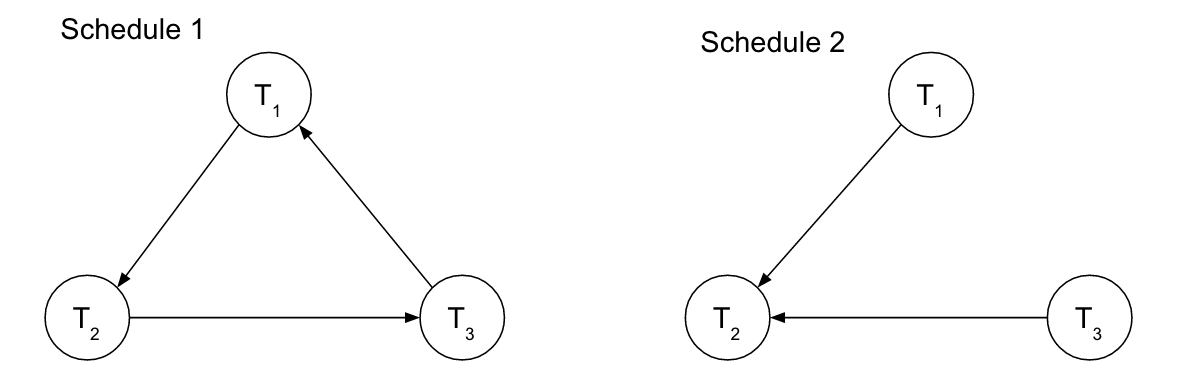
\includegraphics[width=14cm]{graph}
    \caption{Precedence graphs for schedule 1 and schedule 2}
\end{figure} 

As can be seen in the graphs, schedule 1 cannot be syncronized as there is a cycle in the graph. Schedule 2 can be syncronized as it contains no cycle. 

\subsection{Can the schedules be generated using strict 2PL}

To see if the schedules can be generated using strict 2PL we insert the nessesary locks into the schedules, wich can be seen in Figure \ref{fig:schedule1_withlocks} and Figure \ref{fig:schedule2_withlocks}.
In \ref{fig:schedule1_withlocks} we see that when T2 tries to accuire and exclusive lock on X (marked with red in the figure) it has to wait till T1 that alredy has a shared lock on X, finished. This however breaks with the schedule as we see T2 should finish before T1. Schedule 1 therefore could not be generated using strict 2PL. 
In schedule 2 no problems arrise when adding the locks, since T3 finished before T2 need to accuire the shared lock on Z, and T1 finishes before T2 needs the lock on X and Y. So schedule 2 could be generated using strict 2PL. 

\begin{figure}[h]
    \centering
    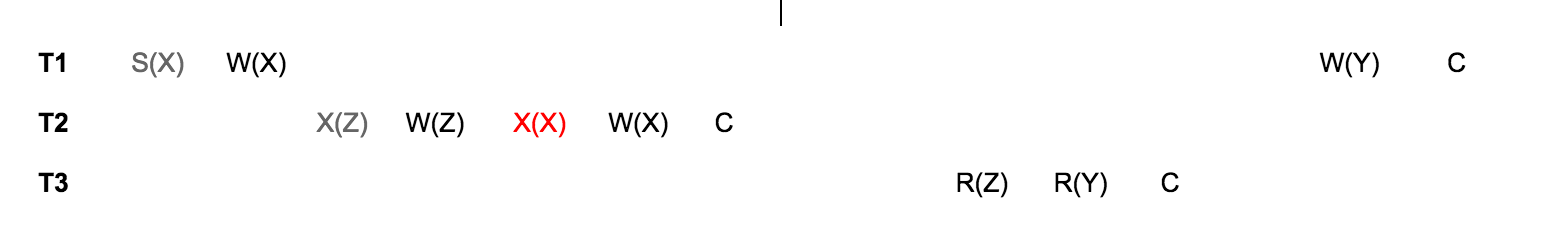
\includegraphics[width=14cm]{schedule1_withlocks}
    \caption{Schedule 1 with locks insterted, S() denotes shared locks, X() denotes explicive locks. In T2 attempt of accuiring the exclusive lock on X that breaks with strict 2PL is shown in red. }
    \label{fig:schedule1_withlocks}
\end{figure} 

\begin{figure}[h]
    \centering
    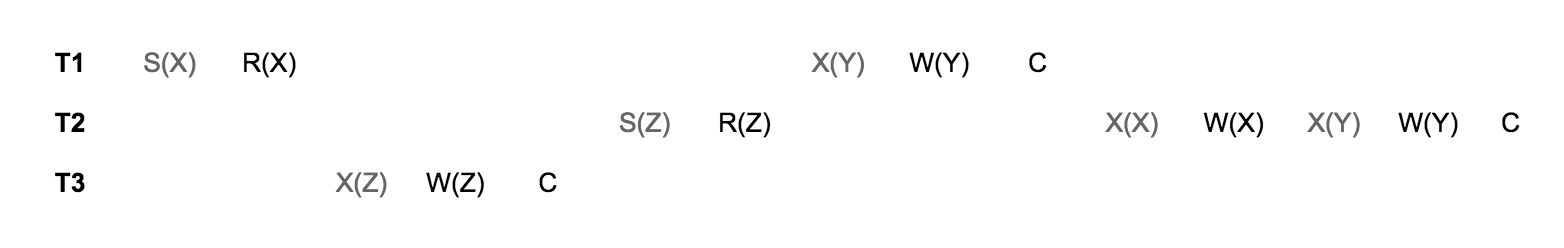
\includegraphics[width=14cm]{schedule2_withlocks}
    \caption{Schedule 2 with locks insterted, S() denotes shared locks, X() denotes explicive locks.}
    \label{fig:schedule2_withlocks}
\end{figure} 

\section{Optimistic Concurrency Control}
In order to see wether T3 are allowed to commit or has to roll back, we write the test for each senario and see if they succeeds or fails. 

\subsection{Scenario 1}

In this senario T3 is not allowed to commit. The reason is that the last check in the test, the union of WS(T2) and RS(T3) is not empty but contain the element $\{4\}$.

\begin{lstlisting}[mathescape]
Test:
   Check that T1 completes before T3 begins
   Check that T2 completes before T3 begins Write phase
   Check that WS(T2) $\cap$ RS(T3) = $\varnothing$
\end{lstlisting}

\subsection{Scenario 2}

T3 is not allowed to commit since the third check in the test, the union of WS(T1) and RS(T3) fails, as the set is not empty but contains the element $\{3\}$.
\begin{lstlisting}[mathescape]
Test:
   Check that T1 completes before T3 begins Write phase
   Check that T2 completes Read phase before T3 completes Read phase
   Check that WS(T1) $\cap$ RS(T3) = $\varnothing$
   Check that WS(T2) $\cap$ RS(T3) = $\varnothing$
\end{lstlisting}

\subsection{Scenario 3}

All checks are possitive so T3 is allowed to commit. 

\begin{lstlisting}[mathescape]
Test:
   Check that T1 completes before T3 begins Write phase
   Check that T2 completes before T3 begins Write phase
   Check that WS(T1) $\cap$ RS(T3) = $\varnothing$
   Check that WS(T2) $\cap$ RS(T3) = $\varnothing$
\end{lstlisting}

\section{Programming task}

\subsection{Short description of implementation and test}
We have used the \verb|ReentrantReadWriteLock| class to implement our locking scheme.

\subsubsection{Strategy}

We acquire a read lock just before validating the input in the methods that are read only, and release it right after reading the result. In the methods that write to the book store map, we acquire a write lock just before validating the input, and hold the lock until the data has been written to the book store. In every method, if an exception is thrown then the held lock is released befre throwing the esception.

\subsubsection{Correctness}

Since we only hold one lock at any point in any method, and that lock is released just before exiting the method, whether through throwing an exception or returning a result, there is not much that can go wrong wih the implementation. This approach makes dirty read and writes impossible, as a method that writes can not be interrupted between validating its input and writing its data. We implemented the test  2 described in the assignment text to test that before-after-atomicity holds up for out implementation, and that no dirty reads happen. Since we validate all input before writing anything, dirty writes are impossible too.

\subsection{Correctness of protocol}



\subsection{Deadlocks}

Deadlocks are not possible in our implementation. Each method only holds one lock, either a read or a write, and a deadlock requires waiting to acquire one or more locks while holding one or more locks. Since each calll to the book store can at most be a series of calls, no thread can hold more than one lock, and that lock will be released before acquiring another, assuring deadlocks are impossible.

\subsection{Scalability bottlenecks}
%Our implementation adheres to strict two-phase locking. 
Because we have used blocking to implement cuncurency there is a scalability bottelneck in regards to the number of clients (transactions), when the transactions begin to conflict and block each. 
When the number of active transactions increase so will the amount of blocking and therefore the amount of delay, which means that throughput will increse more slowly than the number of active transactions. 
In our implementation, we keep locks for a relatively long periode of time and we lock the entire hashmap so the likelyhood of transactions having to wait is fairly big.
If we instead had only locked smaller parts of hashmap, for instance by using a concurrent hashmap (from the java.util.concurrent library) we could have supported both concurrent reads and writes - if the writes was on different parts of the data. This would have made the implementation much more scalable.

\subsection{Overhead}
The amount of concurrency we get depends on wether there is mostly reads or mostly writes in the application. If there are mostly writes there is practically no concurrency, but we still have the overhead due to locking and unlocking. However there is mostly reads or even just some reads the concurrency vs the overhead is pretty good.

\end{document}